This chapter explores the concept of retroactive call subsumption (RCS). RCS
enables full sharing of answers among subgoal calls, independent of the order they are called,
using the relation of subsumption.

First, we introduce the motivations behind RCS by illustrating the shortcomings of traditional call
subsumption mechanisms. Next, we present the concepts introduced by RCS and how execution
rules are extended to support retroactive tabling. Other extensions are then discussed, namely:
the new table space organization based around the ideas of the \textit{common global trie} proposal
\cite{CostaJ-08} and the algorithm to traverse the call trie to search for subsumed subgoals. Finally, we
give some details about the implementation of this new extension in the YapTab system.

\section{Motivation}

In traditional call subsumption, a new call to the subgoal $G$ is considered to create a producer subgoal
when a more general subgoal $G'$ is not found on the call trie and it is the first time $G$ is called.
When $G'$ exists, a new consumer is stored to consume answers from the subsuming subgoal $G'$, thus creating
a consumer subgoal.

Consider that subgoal \texttt{p(X,1,2)} is called first, followed by \texttt{p(X,1,Z)}.
Notice that when \texttt{p(X,1,2)} is called it is considered a producer subgoal as no subsuming subgoals
are found on the call trie. The subgoal \texttt{p(X,1,Z)} is also considered as a producer, because
\texttt{p(X,1,2)} does not subsume \texttt{p(X,1,Z)}. If the call order is swapped, \texttt{p(X,1,Z)} continues
to be considered a producer subgoal, but now \texttt{p(X,1,2)} finds \texttt{p(X,1,Z)} as a subsuming subgoal
on the call trie, and thus is considered a consumer subgoal.

While call subsumption provides good results in terms of memory utilization and time it suffers from a
major problem: the order in which the the subgoals are called can greatly affect the performance
and applicability of the technique. Therefore, we introduce a new mechanism called \textit{retroactive call
subsumption} (RCS) that solves the problem by retroactively modifying active tabled nodes to enable full sharing
of answers between subsuming and subsumed subgoals, independently of the order they are called.

\section{General Idea}

Retroactive Call Subsumption is based around the idea of stopping the computation of subsumed subgoals
that are currently running by transforming those producer subgoals into consumer subgoals, thus instead
of generating their own answers by means of code execution, they will consume answers from the more general
subgoal that has been called.

When the producer subgoal $G$ executes, an arbitrary number of choice points are created that are directly related
to $G$, that is, they are used to compute $G$'s answers. Therefore, when $G$
must be transformed into a consumer subgoal we must \textit{selectively prune} the parts of the computation
that are related to $G$ and transform $G$'s generator choice point in such a way that the choice point
will consume answers from the producer subgoal $G'$, instead of generating its own answers.
Pruning the computation of $G$ can thus potentially save execution time as $G$ no longer properly executes
but consumes answers from another subgoal.

Consider the program in Figure~\ref{fig:retro_program1} that uses RCS and the query goal `\texttt{a(X),~p(Y,Z)}'.
The goal \texttt{a(X)} starts by calling \texttt{p(1,X)}, which succeeds with the answer \texttt{\{X~=~3\}}.
By forward execution, \texttt{p(Y,Z)} is called and verifies if any subsumed subgoal is currently running
and needs to be pruned (Figure \ref{fig:retro_eval1}~(a)). It finds \texttt{p(1,X)} and thus it marks this subgoal frame as a consumer subgoal
frame that will consume from \texttt{p(Y,Z)}.
In order for \texttt{p(1,X)} to act as a consumer, its generator choice point is transformed into
a \textit{retroactive choice point}, which amounts to update the \textit{continuation alternative}
(\texttt{CP\_AP} choice point field) to an instruction called \textit{retroactive\_resolution},
which implements the needed mechanisms to control the evaluation of a \textit{retroactive node}
(Figure \ref{fig:retro_eval1}~(b)).

\begin{figure}[ht]
\begin{Verbatim}
:- use_retroactive_tabling p/2.

a(X) :- p(1, X).

p(1, 3).
p(2, 3).
p(1, 2).
\end{Verbatim}
\caption{Example program using retroactive tabling.}
\label{fig:retro_program1}
\end{figure}

Next, \texttt{p(Y,Z)} continues execution and a new answer is generated, \texttt{\{Y~=~1,~Z~=~3\}}.
By means of backtracking, all answers for \texttt{p(Y,Z)} are generated and the subgoal finally completes.
Execution returns to the retroactive choice point of \texttt{p(1,X)} and retroactive resolution is employed.
As the producer subgoal, \texttt{p(Y,Z)} has already completed, \texttt{p(1,X)} can be turned into a loader
node to consume all answers relevant to the subgoal that were not generated when the subgoal was a generator.
In this case, the only answer available is \texttt{\{X~=~2\}} (Figure \ref{fig:retro_eval1}~(c)).
Note that a retroactive node can be transformed into other types of nodes, as it will become clear in the next
sections.

\begin{figure}[ht]
  \centering
    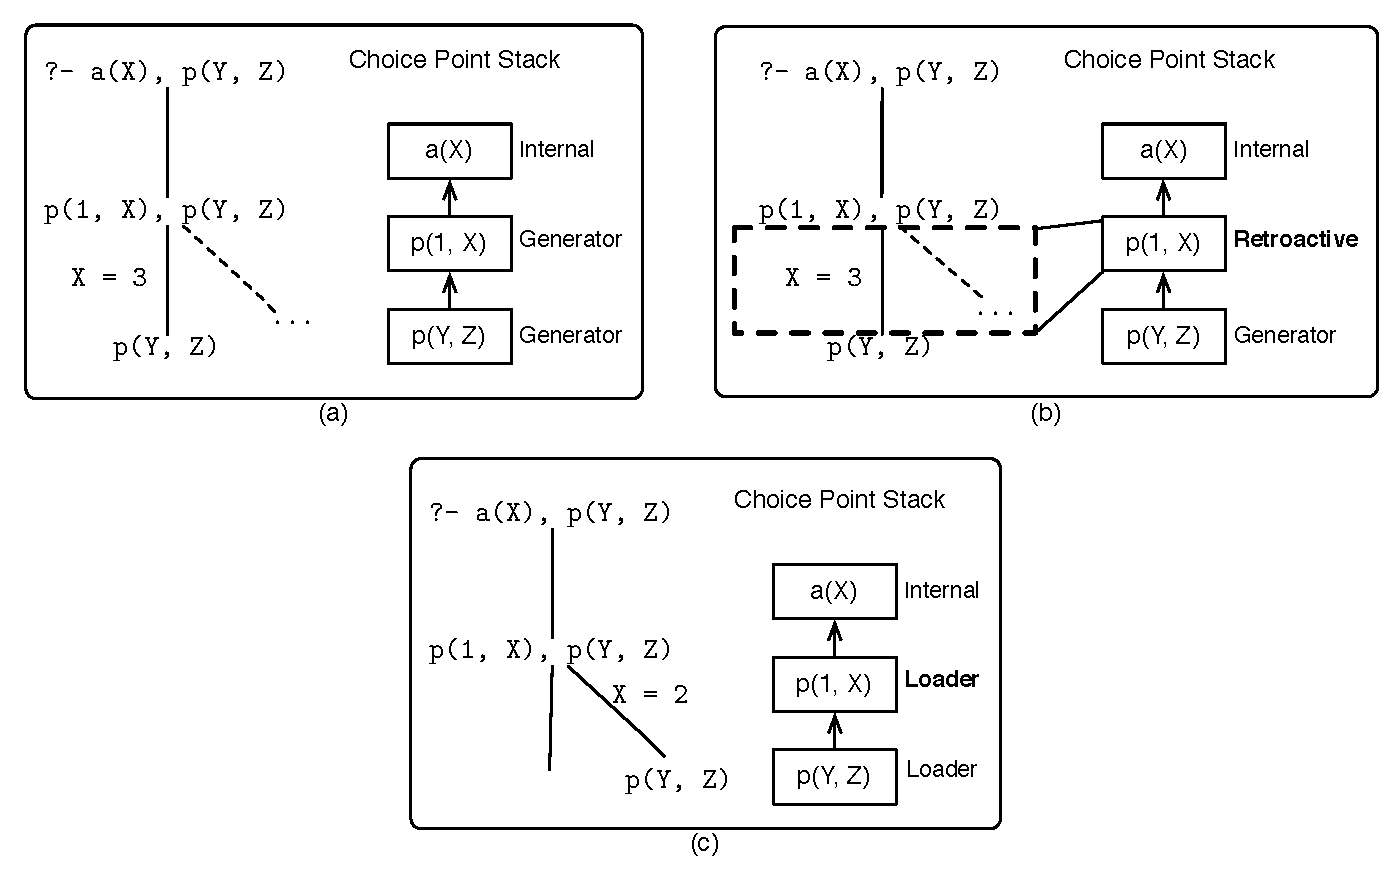
\includegraphics[scale=0.6]{pruning_example1.pdf}
  \caption{Evaluating `\texttt{a(X),~p(Y,Z)}' using retroactive tabling.}
  \label{fig:retro_eval1}
\end{figure}

The previous example has illustrated one special type of pruning called \textit{external pruning}.
External pruning occurs when the subsuming subgoal $G'$ is an \textit{external subgoal} to the evaluation
of the subsumed subgoal $G$. Another type of pruning is called \textit{internal pruning} and happens
when $G'$ is an \textit{internal subgoal} to the evaluation of $G$, that is, $G'$ is called
during the resolution of $G$. Although these two basic types of pruning can derive any other
situation, they both generate the same issues related to evaluation pruning. These issues will be explored
in detail in the next section.

\section{Pruning: Rules and Issues}

When pruning parts of the computation, we must know the areas of the local stack
that contain the choice points to prune. Given the nature of the tabling evaluation, choice points not
directly related to the pruned subgoal can get mixed with other choice points. This happens when a branch
containing external choice points has been suspended, but after backtracking to internal choice points we
execute a subsuming subgoal. Therefore, we must have a mechanism that can tell us if a certain choice
point is internal to a subgoal, from a range of choice points that can potentially contain choice points from
the pruned subgoal.

For this, we construct a dependency tree of subgoals and dependency frames by storing in a field
called \texttt{top\_gen} a pointer to the top tabled subgoal. Thus, by traversing this field we know
what subgoals the target subgoal or consumer is internal to.

When pruning execution branches, issues arise mostly when the computation of the subsumed subgoal involves
consumer and/or generators nodes. The next example programs will illustrate these issues.

Consider the program in Figure~\ref{fig:retro_program2} that mixes tabled predicates using retroactive
call subsumption and tabled predicates with variant checks.
For this program, we will use the query goal `\texttt{a(X,Y),~p(Z,W)}'.

\begin{figure}[ht]
\begin{Verbatim}
:- use_variant_tabling [a/2, b/1].
:- use_retroactive_tabling p/2.

a(X, Y) :- p(1, X), b(Y).
a(3, 4).

b(1).
b(2).

p(1, X) :- a(_, X).
p(1, X) :- b(X).
\end{Verbatim}
\caption{Example program using retroactive tabling with variant tabling.}
\label{fig:retro_program2}
\end{figure}

Initially, evaluation calls \texttt{a(X,Y)} and a new generator node is stored. Next, the retroactive subgoal
\texttt{p(1,X)} is called and creates a new generator node, because no subsuming subgoal is found.
The first clause of \texttt{p/2} executes \texttt{a(\_,X)}, which is a consumer of \texttt{a(X,Y)}, but, as
no answers are available to consume, execution suspends this node and backtracks to try to second clause
of \texttt{p/2}. Here, \texttt{b(X)} is called for the first time, creating a new generator choice point.
An answer for \texttt{b(X)} is generated, \texttt{\{X~=~1\}}, and by forward execution it is also an answer
for \texttt{p(1,X)}. Next, \texttt{b(Y)} is called, creating a new consumer node that consumes the answer
\texttt{\{X~=~1\}} and by forward execution, the first answer for \texttt{a(X,Y)}, \texttt{\{X~=~1,~Y~=~1\}},
is generated.

\begin{figure}[ht]
  \centering
    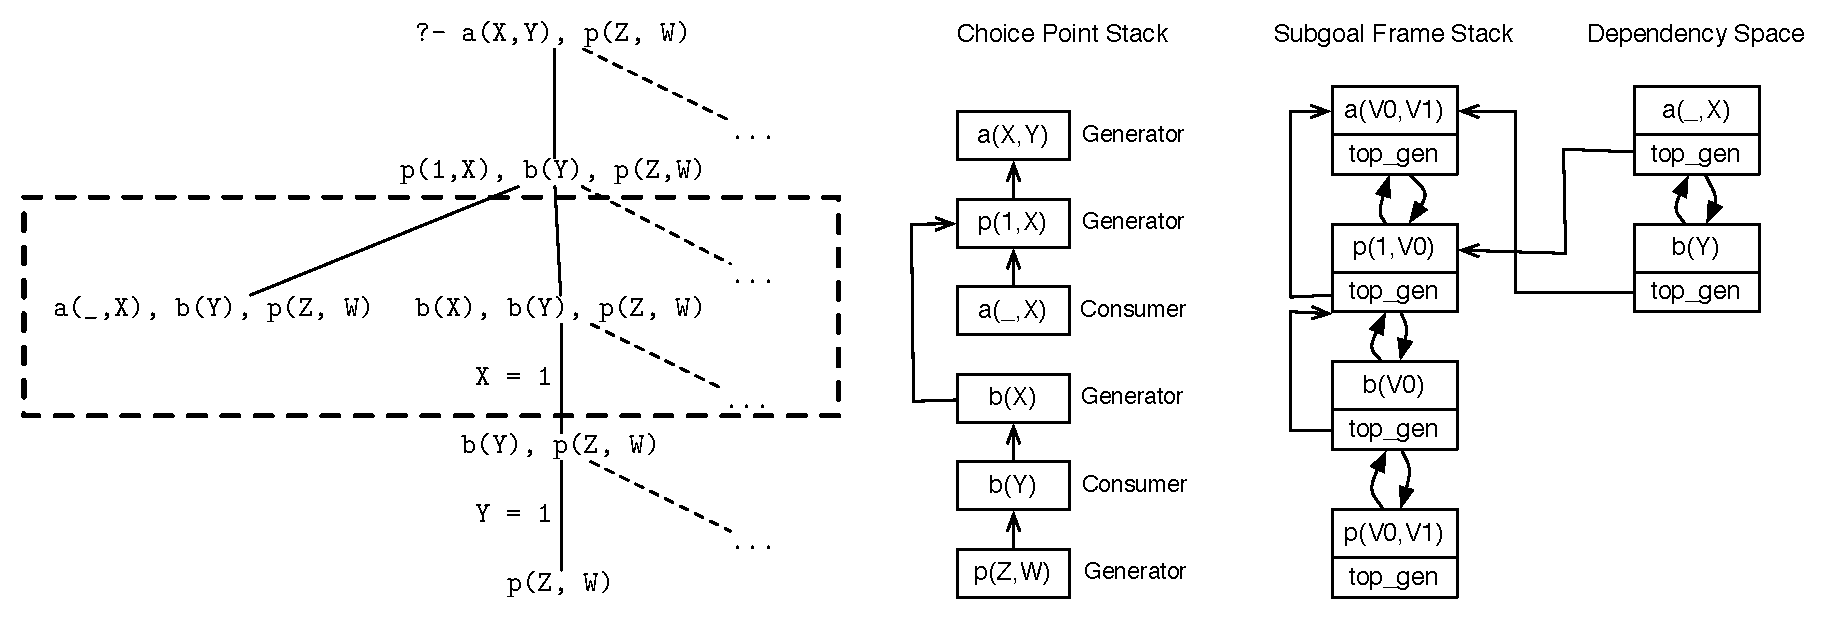
\includegraphics[scale=0.5]{retro_example2.pdf}
  \caption{Evaluating `\texttt{a(X,Y),~p(Z,W)}' using retroactive tabling.}
  \label{fig:retro_eval2}
\end{figure}

Next, subgoal \texttt{p(Z,W)} is called, which subsumes \texttt{p(1,X)} and the evaluation of this subgoal
must be pruned (Figure~\ref{fig:retro_eval2}). As \texttt{p(Z,W)} is external to \texttt{p(1,X)} we have
a case of external pruning. Please notice that \texttt{p(1,X)} now includes various choice
points involved in its computation, namely \texttt{a(\_,X)} and \texttt{b(X)}.

The consumer node associated with the subgoal \texttt{a(\_,X)} must leave the computation and no longer
participates in answer resolution, thus its dependency frame is removed from the dependency space.

Pruning the generator node associated with the subgoal \texttt{b(X)} is a more tricky case. Notice that
the consumer \texttt{b(Y)} depends on this subgoal to consume new answers, thus by removing the generator node
the consumer will become an \textit{orphaned consumer} and the computation will complete too early.
Therefore, we mark the subgoal \texttt{b(X)} as \textit{pruned} and turn the consumer node of \texttt{b(Y)}
into a retroactive node. Finally, the \textit{previous choice point} field of the choice point associated
with \texttt{b(Y)} must now point to \texttt{p(1,X)}, because we must prevent the evaluation to step into
pruned branches by means of backtracking. The choice point of \texttt{b(Y)} is called a
\textit{frontier choice point}. Figure \ref{fig:retro_eval3} shows the state of the computation after pruning.

\begin{figure}[ht]
  \centering
    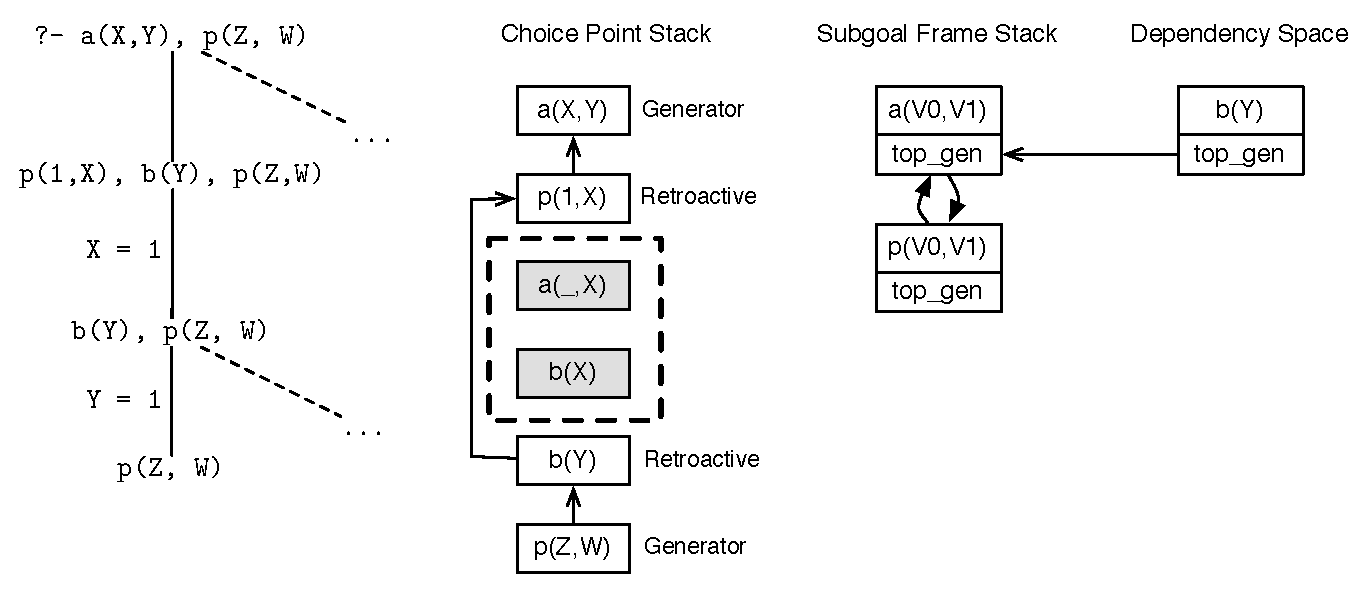
\includegraphics[scale=0.5]{retro_example3.pdf}
  \caption{After external pruning over choice points belonging to the subsumed subgoal.}
  \label{fig:retro_eval3}
\end{figure}

Next, the subgoal \texttt{p(Z,W)} starts to execute the first clause of \texttt{p/2} and creates
a new consumer for \texttt{a(\_,X)}, that will consume one answer. By forward execution, an answer
for \texttt{p(Z,W)}, \texttt{\{Z~=~1,~W~=~1\}}, is generated. By means of backtracking, the second
clause of \texttt{p/2} is executed and calls \texttt{b(Y)}; as \texttt{b(Y)} is a pruned subgoal,
we first load the answers already generated for this subgoal and then execute the clauses of \texttt{b/1}.
After \texttt{b(Y)} generates all the answers, it completes successfully and execution backtracks to
\texttt{p(Z,W)}, to attempt completion of this subgoal. As the leader node is currently \texttt{a(X,Y)},
completion fails.

We backtrack to the retroactive node \texttt{b(Y)} in order to do retroactive resolution. Evaluation
notices that the subgoal has already completed, thus the retroactive node is transformed into a loader node
to consume all answers that were not consumed. By forward execution, a new consumer for \texttt{p(Z,W)} is
created that will generate more answers for the query goal. Once \texttt{b(Y)} does not have more answers
to consume, execution backtracks to the retroactive node of \texttt{p(1,X)}. Here, we note that
the producer subgoal, \texttt{p(Z,W)} has still not completed and this retroactive node must be turned
into a consumer node, which amounts to create a new dependency frame that is added into the dependency space,
in order to participate in the resolution process.

After \texttt{p(1,X)} executes the answer resolution
operation, evaluation backtracks to \texttt{a(X,Y)} that will execute the second clause of \texttt{a/2}.
Once \texttt{a(X,Y)} executes the completion operation and each each consumer has consumed its answers,
the subgoal completes and evaluation is finished.

\subsection{Pruning Actions}

The previous example has illustrated the different actions that must be applied to each choice point that
makes part of the computation of the subsumed subgoal. This action is dependent on the choice point
type and is summarized in the next subsections.

\subsubsection{Interior Nodes}

Interior nodes are related to normal Prolog execution and can be easily pruned
by ignoring them altogether. This approach, while simple, suffers from the problem of \textit{trapped
choice points}. This problem also affects delaying based tabling engines like YapTab and SLG-WAM, where
choice points under consumers are frozen and remain until completion. The CHAT approach to tabling
solves this problem by removing trapped choice points \cite{Demoen-99b}. Another solution would involve
modifications to the WAM garbage collector to collect unused space on the choice point stack.

\subsubsection{Internal Consumers}   
   
Internal consumers must be explicitly pruned by removing the associated
dependency frame from the dependency space. Thus prevents the resolution process to reactivate pruned
branches. In the previous example, \texttt{a(\_,X)} was an internal consumer.

\begin{figure}[ht]
\begin{Verbatim}
abolish_dependency_frames(specific_sg, min, max) {
   top = dependency_frame_before(specific_sg, max)

   while (top != NULL and younger_than(depfr_cons_cp(top), min))
      depfr = top
      top = depfr_next(depfr)

      if (is_internal_depfr(specific_sg, depfr, min))
         remove_from_stack(depfr)
         free(dep_fr)
}
\end{Verbatim}
\caption{Pseudo-code for procedure \texttt{abolish\_dependency\_frames}.}
\label{fig:abolish_dependency_frames}
\end{figure}
   
Figure~\ref{fig:abolish_dependency_frames} shows the procedure that abolishes internal dependency frames.
The arguments are: \texttt{specific\_sg}, the subsumed subgoal to prune; \texttt{min}, the first choice point address from the range of choice points to selectively prune; and \texttt{max}, the last choice point from the pruned range. First, we compute the first dependency frame inside the choice point range by using the function \texttt{dependency\_frame\_before}. Next, we iterate the dependency frames inside the range and check if they are internal to the choice point; if they are, we remove them from the dependency space.

\subsubsection{Internal Generators}

For internal generators we must remove its corresponding subgoal frame
from the subgoal frames stack and alter its state to pruned. Generally, when pruning internal generators, we
have two situations: (1) the generator does not have consumers that are external to the computation of the
subsumed subgoal; or (2) the generator has external consumers. The former situation does not introduce any
problem, but the latter origins orphaned consumers. In our example, the consumer node for \texttt{b(Y)} is
an orphaned consumer.

Usually, a pruned generator is called again during the evaluation of the subsuming subgoal, and before
the computation reaches any of the orphaned consumers. Once reactivated, the subgoal frame for the pruned
generator is pushed again into the top of the subgoal frame stack and its state is altered to
\textit{evaluating}. Then, the new generator node starts by consuming the previously generated answers
and only then executes the program clauses.

\begin{figure}[ht]
\begin{Verbatim}
abolish_subgoal_frames(specific_sg, min, max) {
   top = subgoal_frame_before(specific_sg, max)

   while (top != NULL and younger_or_equal(generator_cp(top), min))
      sg_fr = top
      top = next(sg_fr)

      if (is_internal_subgoal_frame(specific_sg, sg_fr, min))
         sg_cp = generator_cp(sg_fr)
         
         remove_subgoal_from_stack(sg_fr)
         
         if (type(sg_fr) == VARIANT or type(sg_fr) == RETROACTIVE)
            if (has_external_consumers(sg_fr))
               update_external_consumers(specific_sg, sg_fr, sg_cp, max)
               state(sg_fr) = pruned
            else
               free(sg_fr)
         else if (type(sg_fr) == SUBSUMPTIVE)
            if (has_subsumed_consumers(sg_fr))
               transform_external_subsumed_consumers(specific_sg, sg_fr, sg_cp, max,
                  has_variant_consumers(sg_fr))
            
            if (has_variant_consumers(sg_fr))
               update_external_consumers(specific_sg, sg_fr, sg_cp, max)
               state(sg_fr) = pruned
               
            if (has_no_consumers(sg_fr))
               free(sg_fr)
}
\end{Verbatim}
\caption{Pseudo-code for procedure \texttt{abolish\_subgoal\_frames}.}
\label{fig:abolish_subgoal_frames}
\end{figure}

Figure~\ref{fig:abolish_subgoal_frames} shows the procedure \texttt{abolish\_subgoal\_frames} that is
responsible in abolishing internal generators. For variant and retroactive tabled subgoals we remove
the subgoal frame from the stack (using \texttt{remove\_subgoal\_from\_stack}) and then check if the
subgoal has external consumers. If those consumers are found, they are turned into retroactive nodes
by the procedure \texttt{update\_external\_consumers}.

Our system is also able to mix tabled subgoals using traditional call subsumption with retroactive tabling.
For this case we distinguish between variant consumers and subsumed consumers.
If the subgoal has no external variant consumers, we remove the subgoal frame from the system and
its path from the call trie, which means that external subsumed consumers are turned into producers as
the producer has been deleted. When we have external variant consumers, the pruned subgoal changes its state
to \textit{pruned} in order to be reactivated later or by an orphaned consumer.

A tricky situation happens when an orphaned variant consumer is pruned by another subgoal and orphaned
subsumed consumers are left in a situation where the producer subgoal will not be reactivated. In this case,
we check for situations where the subsumptive subgoal has no more variant consumers and we change its state
to \textit{dead}. Later on, when a subsumed consumer is reactivated by means of retroactive resolution, we
verify if the producer is \textit{dead}. If this is the case, we simply convert the subgoal frame to a
subsuming subgoal frame and turn the retroactive node into a generator. This also involves modifications
to the answer template, which must be transformed into a producer answer template (with only variables).

For an example using subsumptive subgoals, consider the program in Figure~\ref{fig:retro_sub} and
the query goal `\texttt{p(1,A),~t(1,2,B),~b(1,C),~p(D,E),~b(F,G)}'.

\begin{figure}[ht]
\begin{Verbatim}
:- use_retroactive_tabling [b/2, p/2].
:- use_subsumptive_tabling t/3.

p(X, 55) :- t(X, A, B).
p(1, 5).
p(10, 10).

b(X, 20) :- t(X, A, B).
b(3, 1).

t(1, 2, 3).
t(1, 2, 5).
t(3, 10, 20).
\end{Verbatim}
\caption{Example program using retroactive tabling with subsumptive tabling.}
\label{fig:retro_sub}
\end{figure}

The first goal \texttt{p(1,A)}
creates a new generator node and calls \texttt{t(1,A,B)}, which is considered a subsumptive producer subgoal.
By forward execution we arrive at \texttt{t(1,2,B)}, which will create a consumer node that subsumes
the subgoal \texttt{t(1,A,B)}. Next, we make another retroactive call with \texttt{b(1,C)} that creates
another generator and calls \texttt{t(1,A,B)}, which is a variant consumer of initial the subsumptive generator.
Finally, we call \texttt{p(D,E)} and \texttt{p(1,A)} must be pruned (Figure~\ref{fig:retro_sub1}).

\begin{figure}[ht]
  \centering
    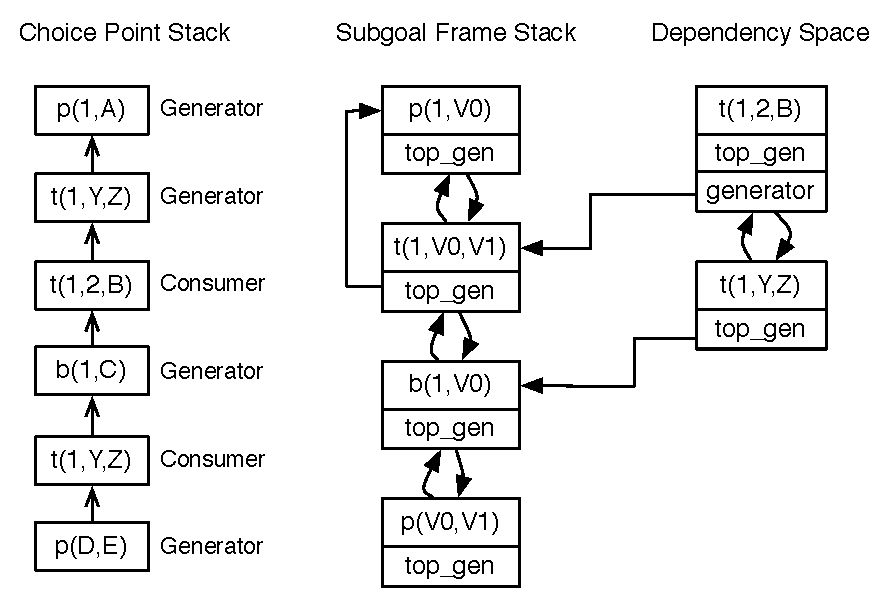
\includegraphics[scale=0.5]{retro_sub1.pdf}
  \caption{Evaluation before pruning subsumptive subgoals using the subgoal \texttt{p(C,D)}.}
  \label{fig:retro_sub1}
\end{figure}

The generator \texttt{t(1,A,B)} is internal to \texttt{p(1,A)} and has two external consumers: one variant
and one subsumed consumer,\texttt{t(1,2,B)}. Here, we modify the state of subsumptive subgoal to \textit{pruned}
and turn each external consumer node into retroactive nodes. We are hoping that \texttt{t(1,A,B)} will be
reactivated and \texttt{t(1,2,B)} will continue to consume from its producer. Figure~\ref{fig:retro_sub2}
shows the state of computation after pruning.

\begin{figure}[ht]
  \centering
    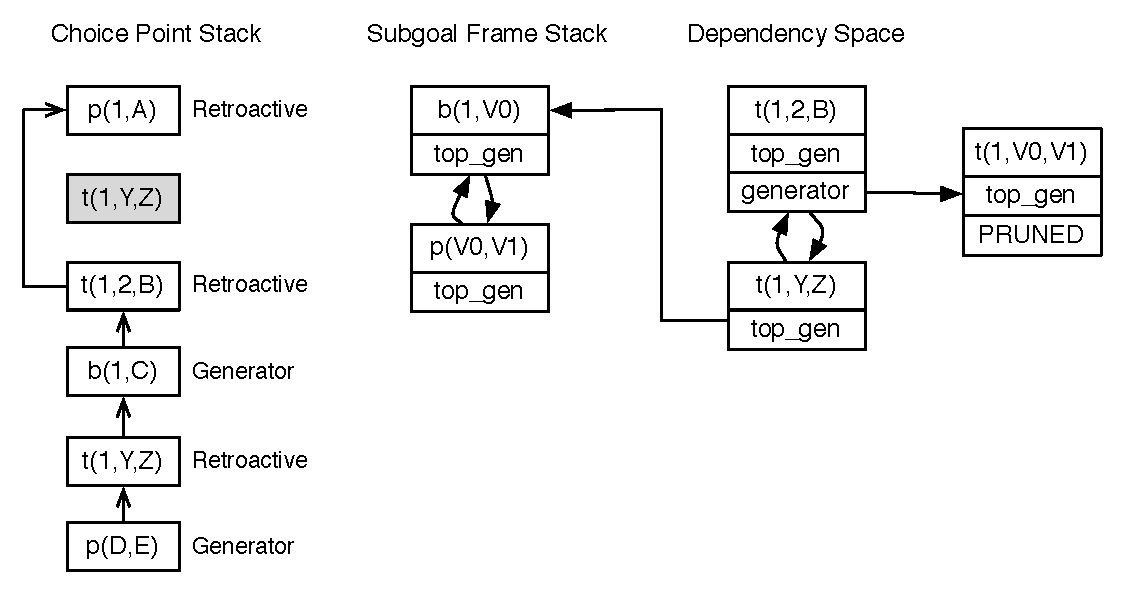
\includegraphics[scale=0.5]{retro_sub2.pdf}
  \caption{Evaluation after pruning subsumptive subgoals using the subgoal \texttt{p(C,D)}.}
  \label{fig:retro_sub2}
\end{figure}

Next, evaluation of \texttt{p(C,D)} generates a call to the subsumptive subgoal \texttt{t(X,A,B)}, which
is a producer subgoal. By forward execution, we call \texttt{b(F,G)} which subsumes \texttt{b(1,C)} and triggers
a new external pruning operation. The computation of \texttt{b(1,C)} contains the internal consumer
\texttt{t(1,A,B)} that is currently associated with a retroactive node. We delete this consumer from the
dependency space and as \texttt{t(1,A,B)} has no more variant consumers that can reactivate this subgoal,
we update its state to \textit{dead}, in order to inform retroactive nodes that dependent on it that the producer
will no longer produce answers (in this example, \texttt{t(1,2,B)}). The result of pruning is shown in
Figure ~\ref{fig:retro_sub3}.

\begin{figure}[ht]
  \centering
    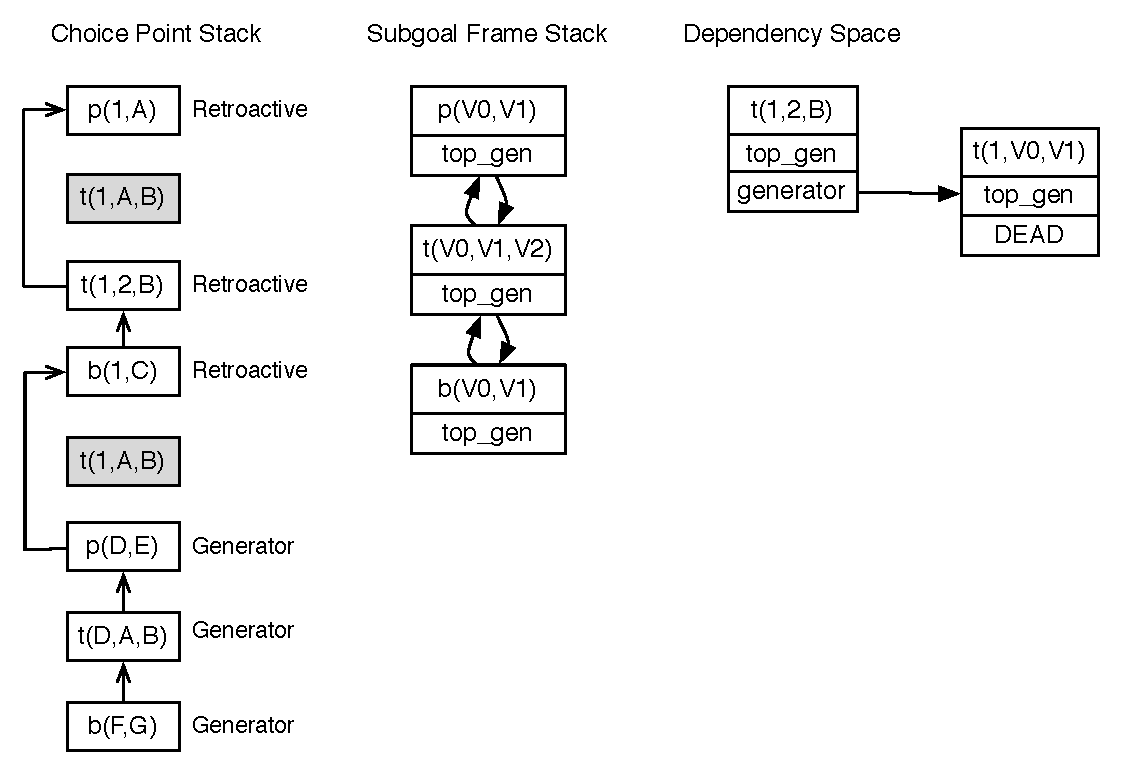
\includegraphics[scale=0.5]{retro_sub3.pdf}
  \caption{Evaluation after pruning subsumptive subgoals using the subgoal \texttt{b(F,G)}.}
  \label{fig:retro_sub3}
\end{figure}

After the subgoals \texttt{b(F,G)}, \texttt{t(X,A,B)} and \texttt{p(D,E)} complete, we backtrack to
the retroactive node \texttt{b(1,C)}. This node is transformed into a loader node as the producer
subgoal has already completed. After the answers have been exhausted, we backtrack to the retroactive
node \texttt{t(1,2,B)}. As the current producer subgoal is \textit{dead} we transform the consumer subgoal
frame into a producer subgoal frame and the retroactive node is transformed into a generator node, because
the subgoal must now generate its own answers. In order for this to work, the answer template is transformed
from \texttt{\{2,~2,~B\}} to \texttt{\{1,~B\}}. Figure \ref{fig:retro_sub4} shows the state of the computation
after this transformation.

\begin{figure}[ht]
  \centering
    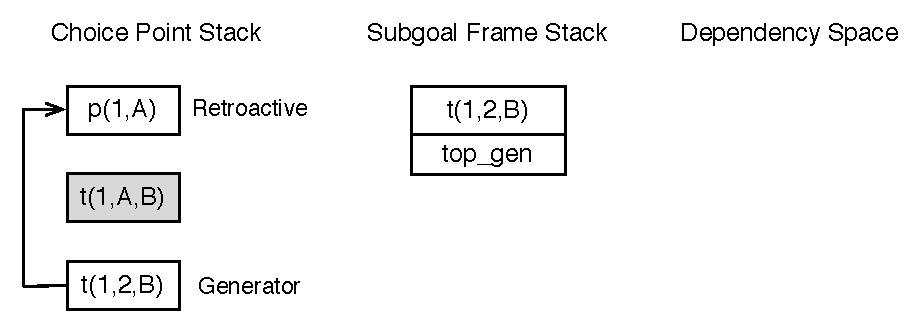
\includegraphics[scale=0.5]{retro_sub4.pdf}
  \caption{Evaluation after transforming the subsumed consumer \texttt{t(1,2,B)} in a subsumptive producer.}
  \label{fig:retro_sub4}
\end{figure}

\subsection{Orphaned Consumers}

An orphaned consumer is an external consumer that loses its generator after a pruning operation.
As we have seen, we transform each orphaned consumer node into a retroactive node.
When an orphaned consumer node is reached by means of backtracking it will be transformed into either:
(1) a loader node, if the pruned generator was reactivated and has completed; (2) a consumer node,
if the pruned generator was reactivated but has not completed yet, which means that below the new pruned subgoal
choice point there is a dependency on a upper generator node, thus this new consumer will participate
in the completion operation as usual; or (3) a generator node,
if the pruned generator was not reactivated until then. This latter situation only occurs with
variant or subsumptive tabling. With retroactive tabling, the execution of the subsuming subgoal
will call the same or a more general subgoal, and this subgoal will update the \texttt{producer} field
of any subsumed subgoal frame, including orphaned consumers.

By default, orphaned consumers always keep their frames on the dependency frame stack. The frame is only
removed if the retroactive node turns into a loader or generator node. If the retroactive node turns again
into a consumer node, lazy removal of dependency frames allows us to avoid removing and allocating a new
frame and the potentially expensive operation of inserting it on the dependency frame stack in the
correct order (ordered by choice point address).

\subsection{Lost Consumers}

While it is usually possible to transform each retroactive node into the correct type of node by means
of backtracking or answer resolution, there are some cases where this is not possible. This happens to
external consumers turned into retroactive nodes and we call them \textit{lost consumers}.

For an example, consider the program in Figure~\ref{fig:retro_lost_consumer_code} and the query goal
`\texttt{a(X,Y)}'. Evaluation starts by storing a generator node for \texttt{a(X,Y)} and then calling
the retroactive subgoal \texttt{p(1,X)}.

\begin{figure}[ht]
\begin{Verbatim}
:- use_variant_tabling [a/2, b/2].
:- use_retroactive_tabling p/2.

a(X, 0) :- p(1, X).
a(0, Y) :- b(1, Y).
a(X, Y) :- p(X, Y).

b(1, Y) :- a(_, Y).
b(2, 1).

p(X, Y) :- b(X, Y).
\end{Verbatim}
\caption{Example program with a lost consumer.}
\label{fig:retro_lost_consumer_code}
\end{figure}

Next, the subgoal \texttt{b(1,X)} is called, creating a new
generator node; consequently \texttt{b(1,X)} calls subgoal \texttt{a(\_,Y)} that is a variant of the
first called subgoal and thus a consumer node is stored. As no answers are available to consume,
evaluation suspends and then backtracks to the second clause of \texttt{b/2}, but it does not
unify with \texttt{b(1,X)}. By backtracking, we attempt the second clause of \texttt{a/2}, which
originates a call to \texttt{b(1,Y)}. This is a variant call of \texttt{b(1,X)} and a new consumer is
created. This node must be suspended as no answers are available.

Through backtracking, we execute the second clause of \texttt{a/2} and the retroactive subgoal \texttt{p(X,Y)}
is called. As this subgoal subsumes \texttt{p(1,X)} we must prune the evaluation of \texttt{p(1,X)}.
The internal generator \texttt{b(1,X)} is pruned, leaving an orphaned consumer, \texttt{b(1,Y)}. The internal
consumer \texttt{a(\_,X)} is simply thrown away. Note that here, we do not have a frontier choice point,
because the subsumed subgoal appears outside the branch of the subsuming subgoal. This is safe, because
the branch including the subsumed subgoal will only be resumed on consumers during completion and thus
no backtracking to previous choice points will occur as they were fully explored before.

After \texttt{p(X,Y)} is fully explored, the following answers are generated for \texttt{a(X,Y)}:
\texttt{\{X~=~1,~Y\}} and \texttt{\{X~=~2,~Y~=~1\}}. Then, we attempt completion at the leader node,
\texttt{a(X,Y)} (Figure~\ref{fig:retro_lost_consumer}). At this point, \texttt{b(1,Y)} still remains
a retroactive node and it is clear that it must be resumed in order to be reactivated as a generator,
and consequently, generate more answers to \texttt{a(X,Y)}, namely \texttt{\{X~=~0,~Y~=~1\}} and
\texttt{\{X~=~0,~Y~=~1\}}. Note that \texttt{b(1,Y)} is not a real consumer and thus can not participate
in the completion operation before retroactive resolution is applied. Therefore, to ensure that all
retroactive nodes are resumed, the completion is extended to, while traversing the dependency space
checking for new answers, also \textit{check for retroactive nodes}, and resume the corresponding
consumer node in both cases. In the example, \texttt{b(1,Y)} is resumed and transformed into a
generator node, thus allowing the computation to finish correctly.

\begin{figure}[ht]
  \centering
    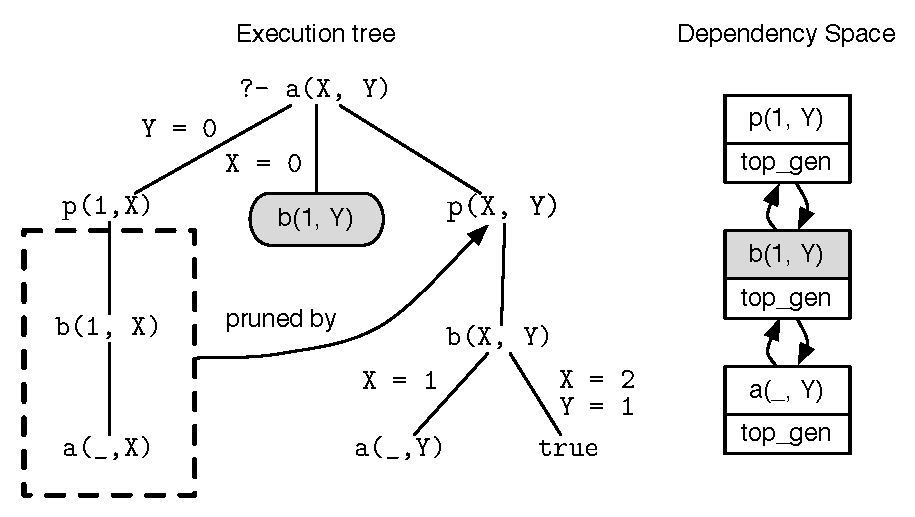
\includegraphics[scale=0.6]{retro_lost_consumer.pdf}
  \caption{Lost consumer \texttt{b(1,Y)} after an external pruning.}
  \label{fig:retro_lost_consumer}
\end{figure}

\subsection{Pseudo-Completion}

When the subsumed subgoal $G$ is pruned when it is a leader node for some consumers, the completion operation
will not be run at node $G$ because $G$ is now a retroactive node and we will not be able to resume
consumers that do not have been fully explored by other leader nodes. Therefore, we must ensure
that every consumer is resumed in order to fully explore every evaluation branch.

Consider the query goal `\texttt{p(1,A,B),~p(1,3,C),~p(D,E,F)}' and the program in Figure~\ref{fig:retro_ignored_consumer}. After the call to \texttt{p(1,A,B)} succeeds with the
answer \texttt{\{A~=~2,~B~=~3\}}, subgoal \texttt{p(1,3,C)} is called and a new consumer of
\texttt{p(A,B,C)} is created (consumer $C1$). As no answers are available to consume, execution
backtracks to \texttt{p(1,A,B)} and a second answer is generated, \texttt{\{A~=~3,~B~=~2\}}. Next,
subgoal \texttt{p(1,3,C)} is called again and a new consumer is generated (consumer $C2$).
This consumers consumes the answer \texttt{\{C~=~2\}} and execution proceeds. 

\begin{figure}[ht]
\begin{Verbatim}
:- use_retroactive_tabling p/2.

p(1, 2, 3).
p(1, 3, 2).
\end{Verbatim}
\caption{Example program for pseudo-completion.}
\label{fig:retro_ignored_consumer}
\end{figure}

Subgoal \texttt{p(D,E,F)} is called and must prune the evaluation of \texttt{p(1,A,B)} 
(Figure~\ref{fig:retro_pseudo_completion1}). Both subgoal frames, \texttt{p(1,A,B)} and \texttt{p(1,3,C)}
are turned into consumer subgoal frames and their \texttt{producer} field is set to the subgoal
frame of \texttt{p(D,E,F)}.

\begin{figure}[ht]
  \centering
    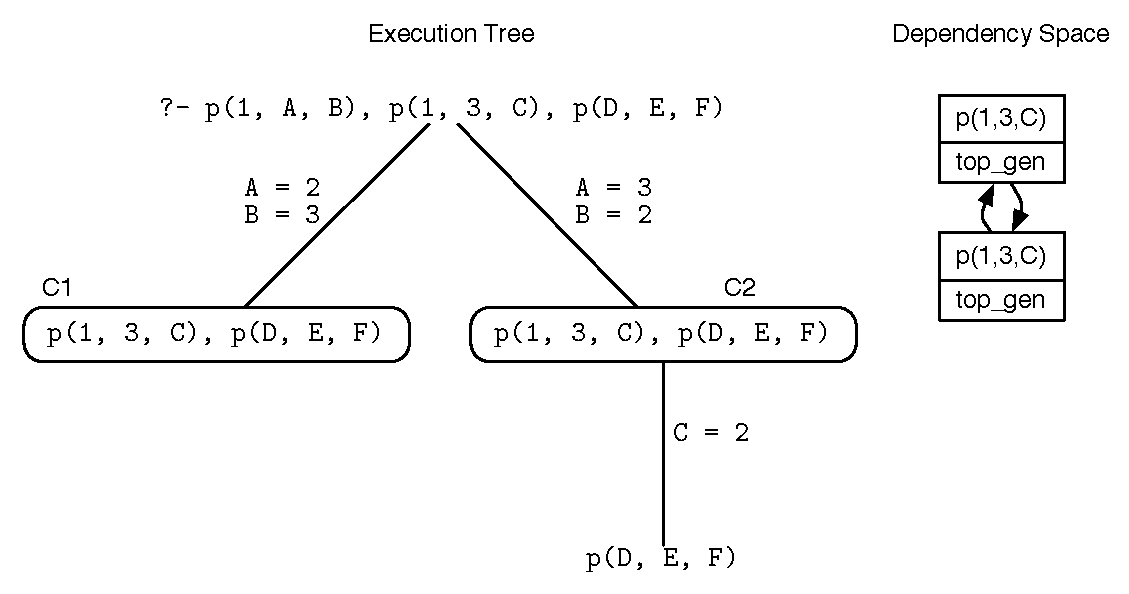
\includegraphics[scale=0.6]{retro_pseudo_completion1.pdf}
  \caption{Query goal `\texttt{p(1,A,B),~p(1,3,C),~p(D,E,F)}' before pruning.}
  \label{fig:retro_pseudo_completion1}
\end{figure}

After \texttt{p(D,E,F)} completes, execution backtracks to retroactive node $C2$ that is transformed
in a loader node by retroactive resolution. After all answers are loaded, execution backtracks to
the retroactive node of \texttt{p(1,A,B)}. If we transform the retroactive node into a loader node and
then load all the answers relevant to this node we might lose the consumer $C1$, because there is no
other way to reach that node.

Notice that when consumer $C1$ has been created its leader node was
\texttt{p(1,A,B)}. Hence, before loading all answers, we act as a \textit{pseudo-leader} (since no upper
dependencies exist) and we look for younger retroactive nodes with unconsumed answers on the dependency
frame stack. When we find node $C1$, we set the field \texttt{backchain\_cp} of the target dependency
frame to the choice point of the pseudo-leader and computation is resumed at $C1$
(Figure \ref{fig:retro_pseudo_completion2}).

After $C1$ is solved
through retroactive resolution, it loads all its answers and, instead of backtracking, jumps to the choice
point saved in the \texttt{backchain\_cp} field, thus allowing the pseudo-leader to resume other retroactive
nodes. The reason to use the \texttt{backchain\_cp} field instead of backtracking, is because any choice
point between the pseudo-leader and the target consumer as been fully exploited, thus we must jump explicitly
between nodes. The process of resuming consumers through a pseudo-leader is called \textit{pseudo-completion}.

\begin{figure}[ht]
  \centering
    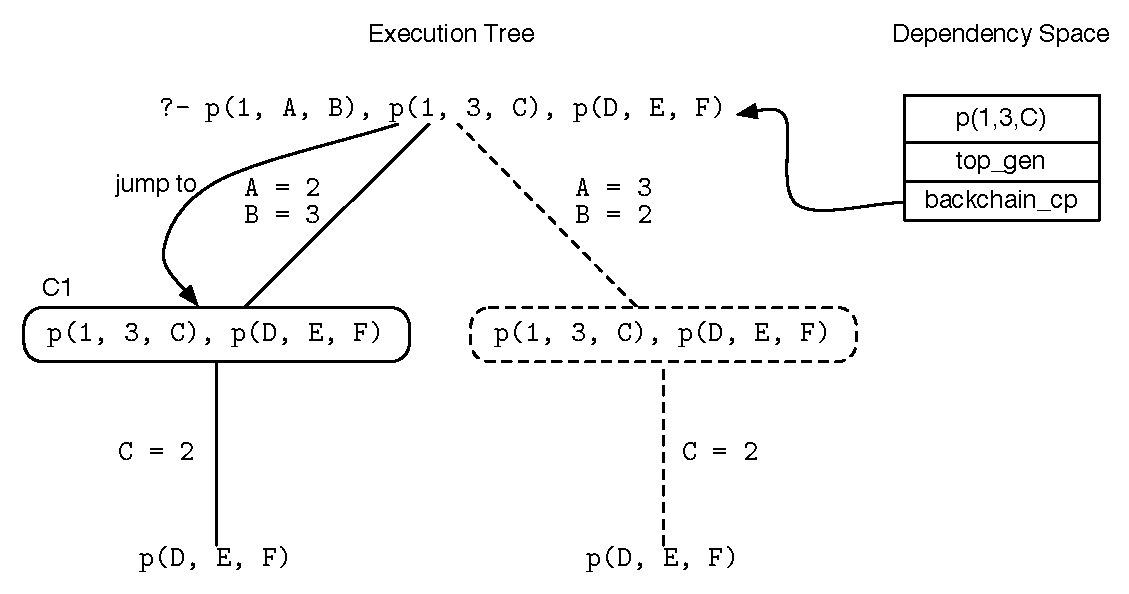
\includegraphics[scale=0.6]{retro_pseudo_completion2.pdf}
  \caption{Executing a pseudo-completion.}
  \label{fig:retro_pseudo_completion2}
\end{figure}

\subsection{Leader Re-Computation}

Each dependency frame contains the value of the leader node during the creation of the consumer node.
External consumers can reference as a leader either: (1) a pruned generator choice point; or (2) a
generator that appeared before the execution of the subsumed subgoal. In the second case we keep
the dependency frame unmodified. In the first case, we update the leader choice point (\texttt{leader\_cp})
field to the consumer node itself.

The reason we update the \texttt{leader\_cp} field is to avoid the leader computation algorithm to compute
a leader that simply does not exist, making completion impossible.
For an example describing this problem, consider the program in Figure~\ref{fig:retro_leader_program}
and the query goal `\texttt{p(1,A),~a(B,C),~a(1,D),~p(E,F)}'.

\begin{figure}[ht]
\begin{Verbatim}
:- use_retroactive_tabling p/2.
:- use_variant_tabling p/2.

a(1, 3).
a(1, 2).
a(2, 4).

p(X, Y) :- a(X, Y).
\end{Verbatim}
\caption{Example program demonstrating the leader re-computation problem.}
\label{fig:retro_leader_program}
\end{figure}

During the evaluation of the subgoal \texttt{p(1,A)}, a generator node
for \texttt{a(1,Y)} is created. Next, a new generator is allocated for \texttt{a(B,C)},
followed by the consumer node \texttt{a(1,D)}. When \texttt{p(E,F)} is called to
prune \texttt{p(1,A)} (Figure~\ref{fig:retro_leader_recomputation}), the generator \texttt{a(1,Y)}
is pruned and the \texttt{leader\_cp}
field of the consumer \texttt{a(1,D)} still points to \texttt{a(1,Y)}.
During execution of \texttt{p(E,F)} a new consumer is allocated for \texttt{a(X,Y)} that
decides its leader should be the pruned \texttt{a(1,X)} generator, because between
the generator and consumer nodes, the \texttt{a(1,D)} consumer has an older leader.

\begin{figure}[ht]
  \centering
    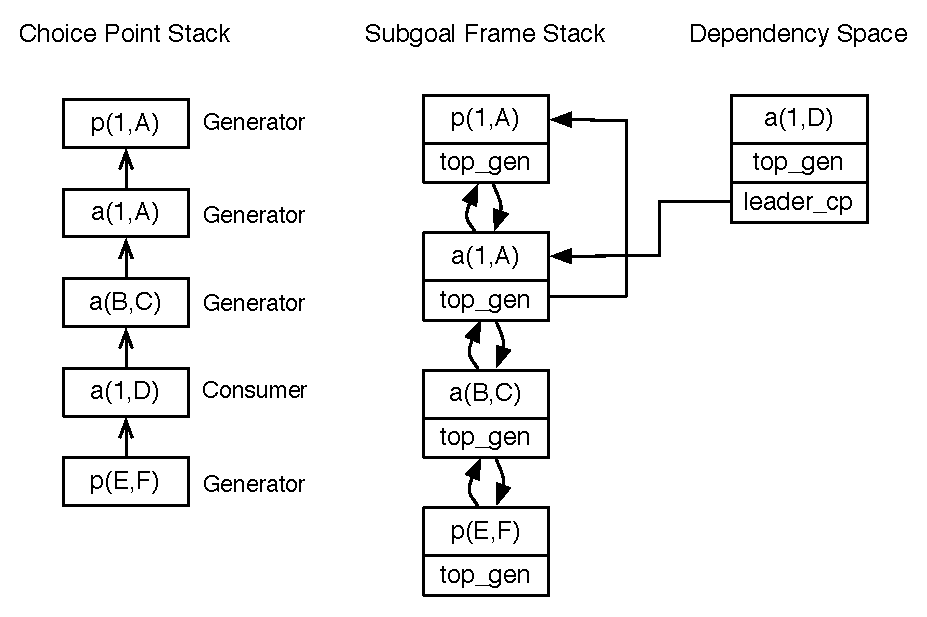
\includegraphics[scale=0.6]{retro_leader_recomputation.pdf}
  \caption{Before pruning the subsumed subgoal.}
  \label{fig:retro_leader_recomputation}
\end{figure}

Finally, execution proceeds and completion is attempted at the subgoal \texttt{p(E,F)}.
Because this is not the leader node, we backtrack to \texttt{a(1,D)} that is transformed
into a generator and then completes. Next, we backtrack to \texttt{a(B,C)} to try other
alternatives of \texttt{a/2} and then completion is attempted, but without success because
the leader node is the pruned generator \texttt{a(1,Y)}. It is then impossible to complete
the evaluation because the leader node is never reached.

By our delineated rules, the \texttt{leader\_cp} of the consumer \texttt{a(1,D)} would have been
modified to itself, thus making the generator \texttt{a(B,C)} the leader of the computation.
Notice that the consumer node, \texttt{X,Y} created during the evaluation of \texttt{p(E,F)} would
consider that its leader was \texttt{a(B,C)}. Figure~\ref{fig:retro_leader_recomputation2} shows the
state of computation at that point.

\begin{figure}[ht]
  \centering
    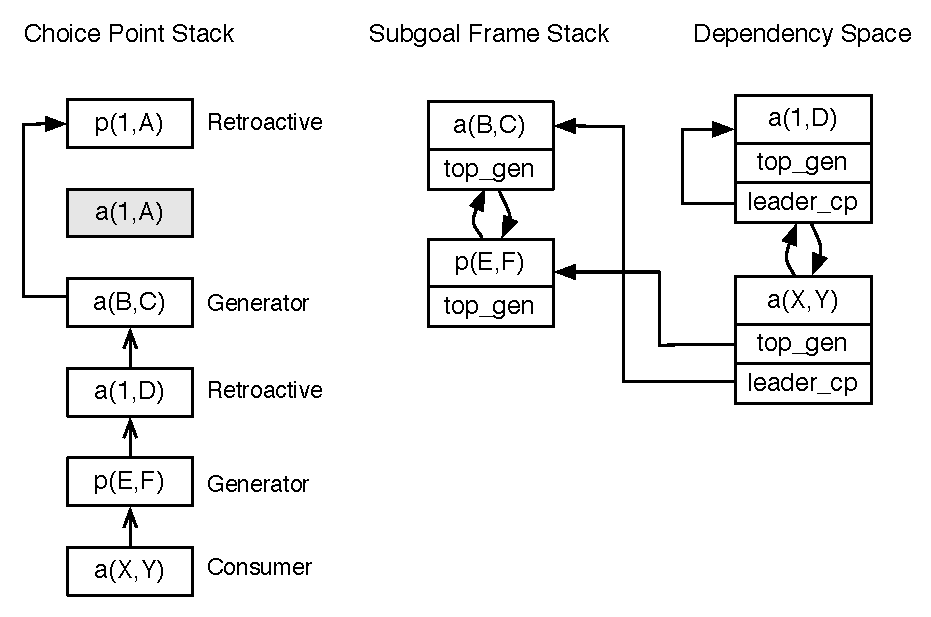
\includegraphics[scale=0.6]{retro_leader_recomputation2.pdf}
  \caption{Updated \texttt{leader\_cp} fields.}
  \label{fig:retro_leader_recomputation2}
\end{figure}

\section{Internal Pruning}

Although all the previous example used external pruning, both external and internal pruning
suffer from the issues previously described. This section explores internal pruning
and its differences in relation to external pruning.

Internal pruning occurs when the subsuming subgoal $S$ is internal to the evaluation of the
subsumed subgoal $R$. In this type of pruning we want to keep one part of $R$ running, the one
that computes $S$, hence we are able to compute all answers of $R$ just by computing $R$.

Our approach involves computing $S$ using local scheduling \cite{Freire-96}, but without returning
answers to the environment of $R$, as it has been pruned. Instead, we jump directly to the
choice point of $R$, which was transformed into a retroactive, and resume the computation there
in order to consume the matching answers found by $S$. When resuming the retroactive node for $R$, it
can become either: (1) a loader node, if $S$ has completed; or (2) a consumer node, if $S$ has not
completed because it is not the leader node, i.e., the leader node is above $R$.

Notice that, when the completion operation is later attempted at the leader node, the computation can
still be resumed, as usual and without any special handling, at $R$ or at the internal consumers of $S$,
until no unconsumed answers are available.

For an example, consider the \texttt{path/2} program presented in Figure~\ref{fig:retro_path_program}.
It computes the reachability between two nodes on a directed graph by using a left recursive
definition. To know from which nodes we can reach node 3, we are interested in the solutions
for the query goal `\texttt{path(X,3)}'.

\begin{figure}[ht]
\begin{Verbatim}
:- use_retroactive_tabling path/2.

path(X, Y) :- path(X, Z), edge(Z, Y).
path(X, Y) :- edge(X, Y).

edge(1, 2).
edge(2, 3).
\end{Verbatim}
\caption{Left recursive \texttt{path/2} program with retroactive tabling.}
\label{fig:retro_path_program}
\end{figure}

Execution starts by creating a generator node for \texttt{path(X,3)}, followed by a call to
subgoal \texttt{path(X,Z)}. Given that \texttt{path(X,Z)} is internal to the computation of
\texttt{path(X,3)}, we have a case of internal pruning. Using the rules for internal pruning
defined above, we will evaluate \texttt{path(X,Z)} with local scheduling.

Next, a repeated call to the subgoal \texttt{path(X,Z)} is made and a consumer is created.
As no answers are available for consumption, execution backtracks to the second clause of \texttt{p/2}.
Here, we call \texttt{edge(X,Y)} and two new answers for \texttt{path(X,Z)} are generated,
\texttt{\{X~=~1,~Z~=~2\}} and \texttt{\{X~=~2,~Z~=~3\}}. Execution returns to \texttt{path(X,Z)} and
completion is attempted. As the \texttt{path(X,Z)} consumer now has answers to consume, they are
thus consumed and by forward execution the solution \texttt{\{X~=~1,~Z~=~3\}}  is generated for
\texttt{path(X,Z)}. Notice that these answers are not returned to the environment of
\texttt{path(X,3)}, but are only saved on the table space.

After a batch of repeated answers, execution backtracks to \texttt{path(X,Z)} where
completion is attempted again (Figure~\ref{fig:retro_path}). With no more unconsumed answers, the subgoal
\texttt{path(X,Z)} completes and instead of backtracking, jumps to the retroactive node of the subgoal
\texttt{path(X,3)}. Here, the retroactive node first determines the relevant answers from the set of
answers generated for \texttt{path(X,Z)}, namely, \texttt{\{X~=~1\}} and \texttt{\{X~=~2\}}. Next,
the retroactive node is transformed into a loader node, thus loading its answers.

\begin{figure}[ht]
  \centering
    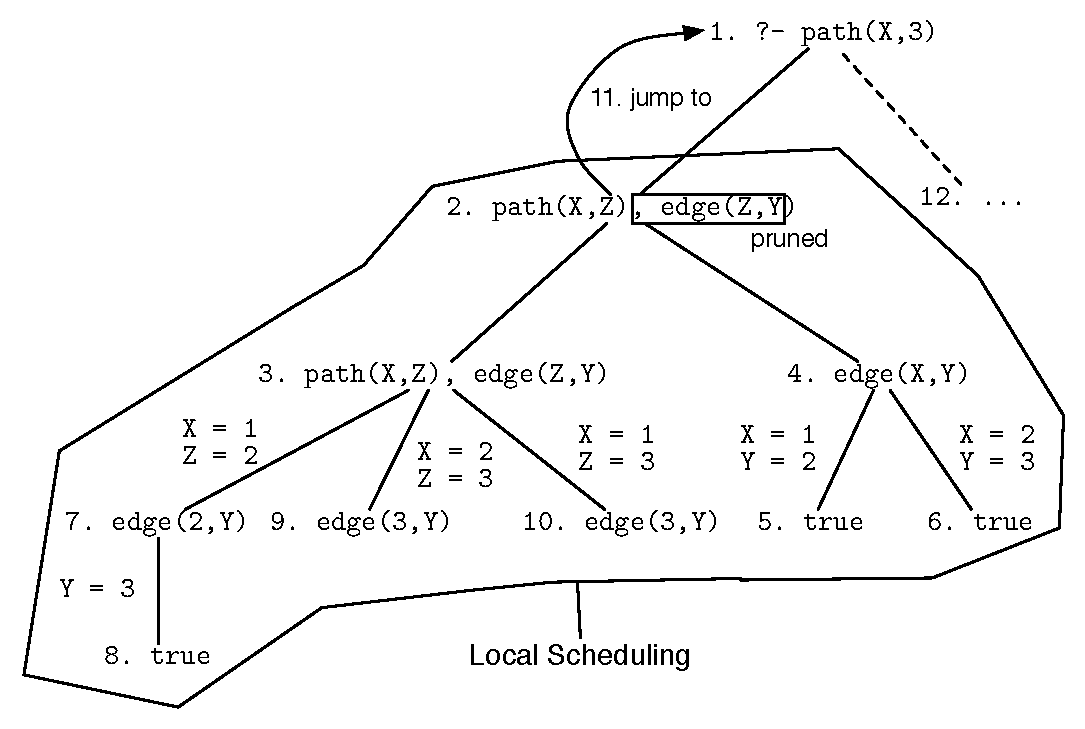
\includegraphics[scale=0.7]{retro_path.pdf}
  \caption{Evaluating `\texttt{path(X,3)}' using retroactive tabling.}
  \label{fig:retro_path}
\end{figure}

\subsection{Multiple Internal Pruning}

An important aspect in internal pruning is \textit{multiple internal pruning}.
Consider that a subgoal $R_1$ calls recursively internal subgoals $R_1, R_2, ..., R_n$ until a subgoal
$S$ is called that subsumes $R_1, R_2, ..., R_n$. In such cases, we ignore all intermediate subgoals
and answers are only pushed from $S$ to $R_1$, the top subgoal. 
For an example, consider the query goal `\texttt{p(1,X)}' and the program in Figure~\ref{fig:retro_multiple_internal_program}.

\begin{figure}[ht]
\begin{Verbatim}
:- use_retroactive_tabling p/2.

p(1,X) :- p(2,X).
p(2,X) :- p(X, _).
p(2,4).
p(1,5).
\end{Verbatim}
\caption{Example program illustrating multiple internal pruning.}
\label{fig:retro_multiple_internal_program}
\end{figure}

Execution starts by storing generator nodes for \texttt{p(1,X)} and \texttt{p(2,X)} and then
\texttt{p(2,X)} calls \texttt{p(X,\_)} that subsumes both \texttt{p(1,X)} and \texttt{p(2,X)}.
Pruning is done between the top subsumed subgoal \texttt{p(1,X)} and the subsuming subgoal
\texttt{p(X,\_)} and the node for \texttt{p(2,X)} is ignored (Figure~\ref{fig:retro_multiple_internal1}).
The choice point for \texttt{p(1,X)} is transformed into a retroactive node and execution proceeds by
applying local scheduling to evaluate \texttt{p(X,\_)}.

\begin{figure}[ht]
  \centering
    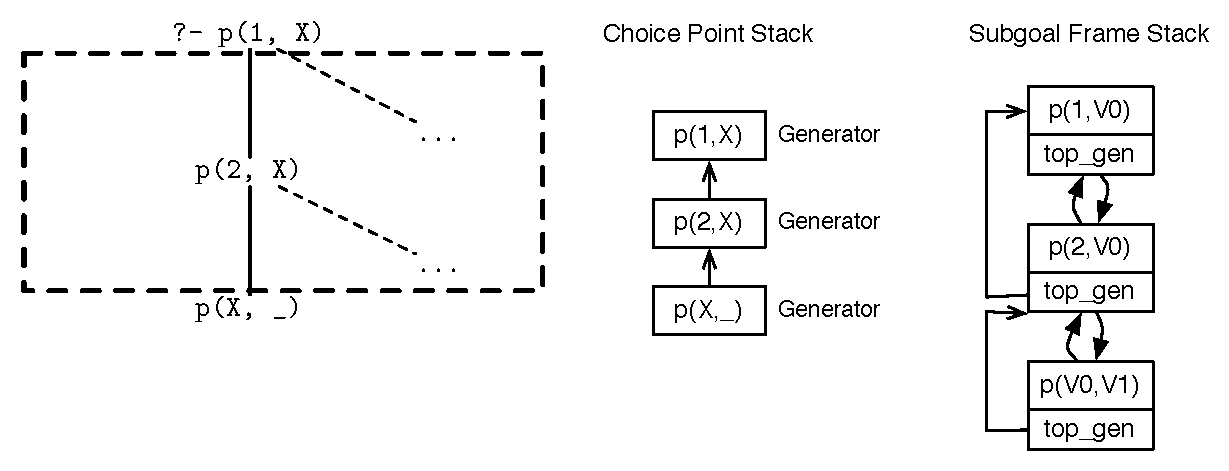
\includegraphics[scale=0.6]{retro_multiple_internal1.pdf}
  \caption{Before multiple internal pruning.}
  \label{fig:retro_multiple_internal1}
\end{figure}

After \texttt{p(X,\_)} fully evaluates with the answers \texttt{\{X~=~1\}}, \texttt{\{X~=~2\}},
\texttt{\{X~=~2,~\_~=~4\}} and \texttt{\{X~=~1,~\_~=~5\}}, execution is resumed at the retroactive node of
subgoal \texttt{p(1,X)}, where the answers \texttt{true} and \texttt{\{X~=~5\}} are loaded
(Figure~\ref{fig:retro_multiple_internal2}).
While the subgoal \texttt{p(2,X)} did not participate in later phase of the computation, it has been completed
during the computation of \texttt{p(X,\_)}. 

\begin{figure}[ht]
  \centering
    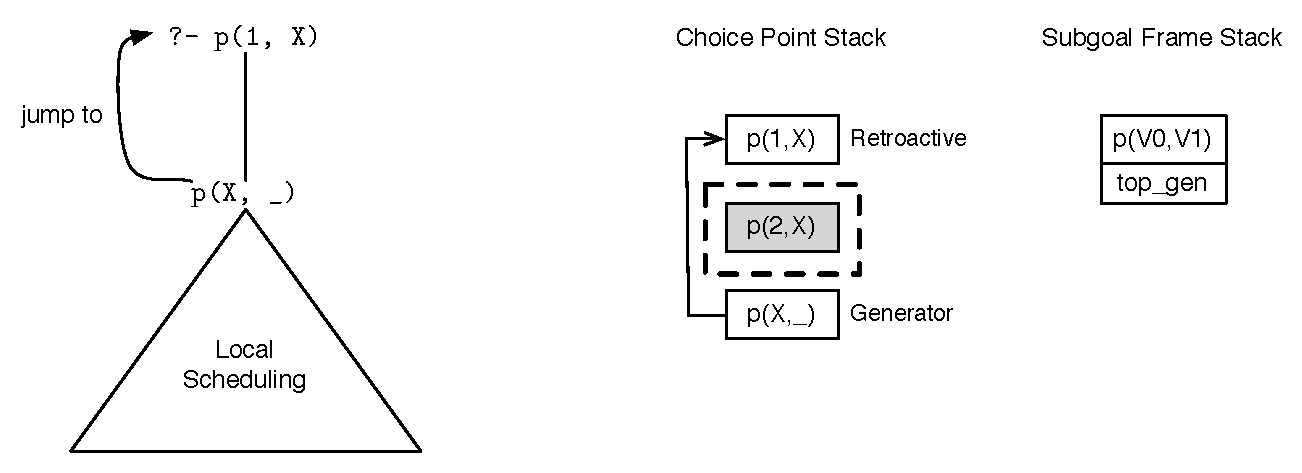
\includegraphics[scale=0.6]{retro_multiple_internal2.pdf}
  \caption{After the evaluation of \texttt{p(X,\_)}.}
  \label{fig:retro_multiple_internal2}
\end{figure}

\section{Mixing External and Internal Pruning}

Although internal and external pruning form the basis of retroactive call subsumption, rules must
be devised in order to prune multiple subgoals that combine both types of pruning. We want to
the minimize the number of pruned subgoals in such a way that a choice point is pruned at
most one time.

Figure~\ref{fig:prune_subgoal_list} shows the \texttt{prune\_subgoal\_list} procedure that accepts
as arguments the subsuming subgoal and the list of subgoals to prune.

First, we compute the oldest internal subgoal $O$ in the set of subgoals and discard other internal
subgoals (phase 1). By using the multiple internal pruning principle (Observation \ref{internal_obs}), we can prune only the oldest subgoal
because pruning the oldest subgoal will also prune the other internal subgoals as a side-effect.
Notice that we also change the subgoal frame type of all subsumed subgoals to \texttt{RETROACTIVE\_CONSUMER}
and update the \texttt{producer} field to point to the subsuming subgoal.

\begin{pruning_obs}\label{internal_obs}
Let $R_1, R_2, ..., R_n$ be a set of subgoals that are recursively internal. In order to prune the subgoals
$R_1, R_2, ..., R_n$, only the top subgoal, $R_1$, needs to be pruned.
\end{pruning_obs}

Next, in phase 2 we check if the list of subgoals is empty, that is, if no external subgoals exist in the list
because internal subgoals have been removed from it in phase 1. Affirmatively, we return early from the procedure
by doing an internal pruning.

In phase 3, we remove all internal subgoal frames that are internal to the subgoal frame $O$ found in phase 1.
Because we will prune the computation of $O$, every subgoal internal to $O$ will be pruned
(except the subsuming subgoal), thus there is no need to prune the two subgoals separately
(Observation~\ref{external_obs}). Next, we finally do an internal pruning using the $O$ subgoal frame
and the resulting list at this point will be empty or contain only external subgoal frames not internal to
$O$ where external pruning must be applied.

\begin{pruning_obs}\label{external_obs}
Let $G$ be a subgoal and $G'$ a subgoal internal to $G$. If $G$ is pruned, $G'$ is also pruned.
\end{pruning_obs}

If the list of subgoals is not empty, we iterate over each external subgoal frame to remove the subgoal frame if
it is internal to another one in the list (phase 4). This is also based on Observation~\ref{external_obs}.
Finally, in phase 5 we apply external pruning to each remaining external subgoal.

For an example, consider the program in Figure~\ref{fig:retro_mix_program} and the query goal
`\texttt{p(2,X),~p(4,Y)}'. Initially, execution creates the generator \texttt{p(2,X)} followed by the internal
generator \texttt{p(3,X)}. Next, the subgoal \texttt{p(4,Y)} is called and the first alternative calls the
subgoal \texttt{p(\_,Y)}, which subsumes every other subgoal (Figure~\ref{fig:retro_mix_multiple_before}).

\begin{figure}[ht]
\begin{Verbatim}
:- use_retroactive_tabling p/2.

p(2, X) :- p(3, X).
p(2, 1).
p(3, 2).
p(3, 5).
p(4, X) :- p(_, X).
p(4, 7).
\end{Verbatim}
\caption{Example program illustrating multiple pruning.}
\label{fig:retro_mix_program}
\end{figure}

By following the rules we previously defined, the oldest internal subgoal we find is \texttt{p(4,X)}.
Next, we filter subgoals that are internal to \texttt{p(4,X)}, but no such subgoals exist. Computation is
then internally pruned by the subgoal \texttt{p(4,X)} and then we must deal with external subgoals.

\begin{figure}[ht]
  \centering
    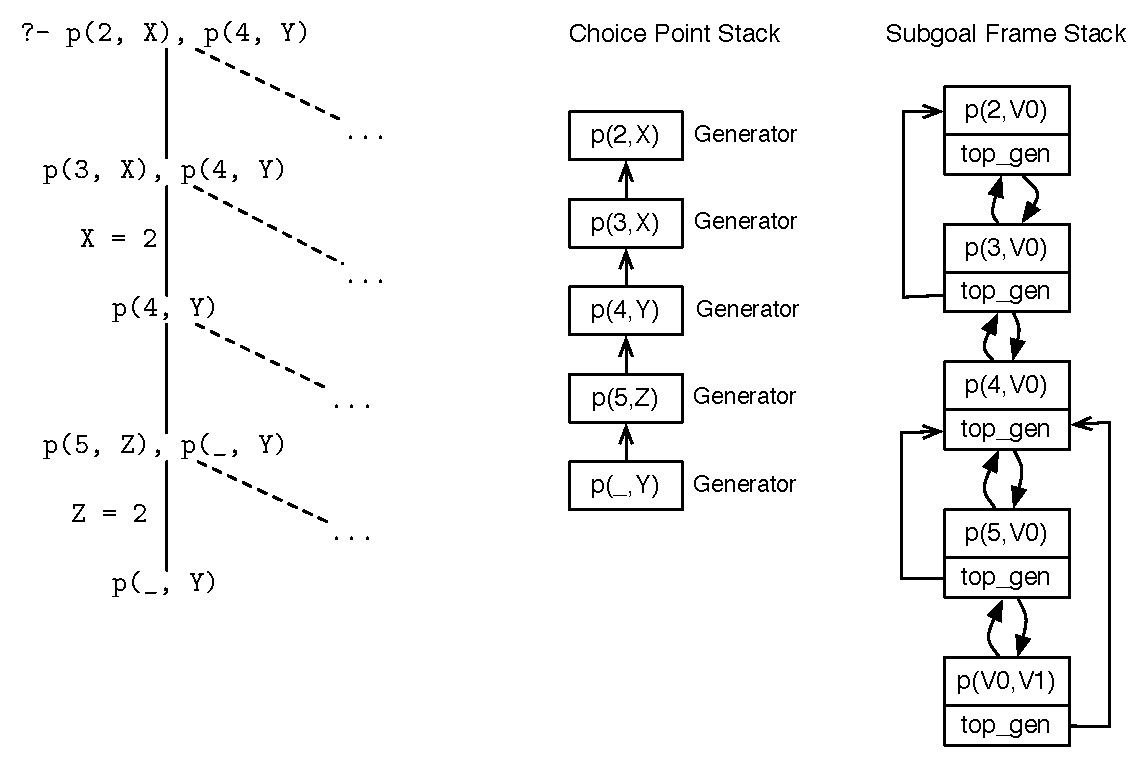
\includegraphics[scale=0.6]{retro_mix_multiple_before.pdf}
  \caption{Before pruning with the subgoal \texttt{p(\_,Y)}.}
  \label{fig:retro_mix_multiple_before}
\end{figure}

The remaining external subgoals are \texttt{p(2,X)} and \texttt{p(3,X)}. Here we must ignore any subgoal
that is internal to any external subgoal. The subgoal \texttt{p(3,X)} matches these conditions and, is thus
removed. Finally, the only remaining subgoal, \texttt{p(2,X)}, is then externally pruned and the computation
can continue as normal.

\begin{figure}[ht]
  \centering
    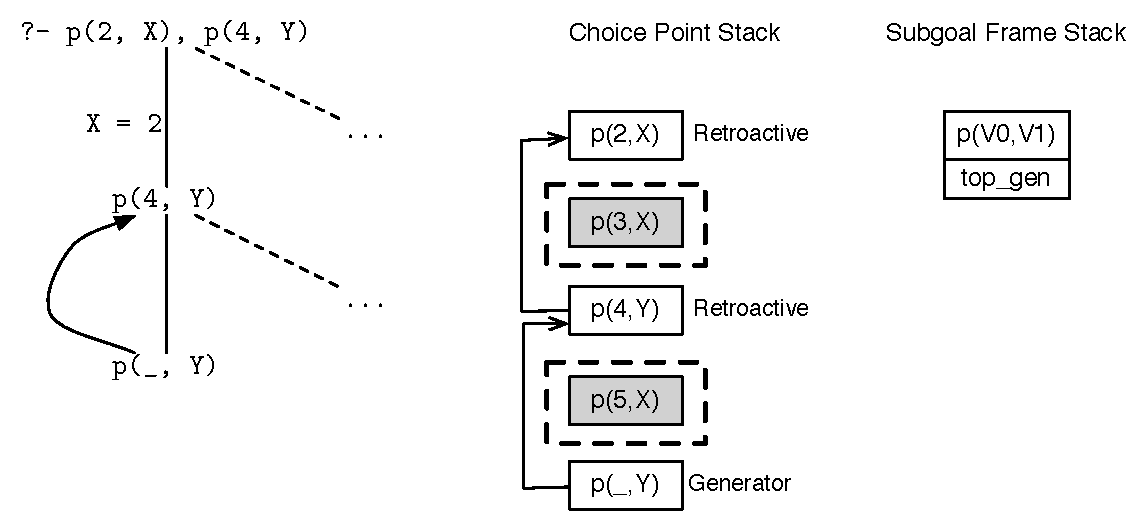
\includegraphics[scale=0.6]{retro_mix_multiple_after.pdf}
  \caption{After pruning with the subgoal \texttt{p(\_,Y)}.}
  \label{fig:retro_mix_multiple_after}
\end{figure}



\begin{figure}[ht]
\begin{Verbatim}
prune_subgoal_list(subsuming, list) {
  if (empty(list))
    return
    
  // phase 1: locate oldest internal subgoal to prune
  min_internal_sg = NULL
  foreach (subgoal in list)
    // change type of subgoal frame and producer
    type(subgoal) = RETROACTIVE_CONSUMER
    producer(subgoal) = subsuming
    
    if (is_internal(subgoal))
      if (min_internal_sg == NULL or
            older_than(generator_cp(subgoal), generator_cp(min_internal_sg)))
        min_internal_sg = subgoal
      
      remove_from_list(list, subgoal)
  
  // only external subgoals in 'list'
  
  // phase 2: return early by checking the existance of external subgoals
  if (empty(list))
    // no external subgoals
    internal_prune(subsuming, min_internal_sg)
    return
  
  if (min_internal_sg)
    // phase 3: filter external subgoals internal to 'min_internal_sg'
    foreach (subgoal in list)
      if (is_internal_subgoal_frame(min_internal_sg))
        remove_from_list(list, subgoal)
    
    // internal prune with 'min_internal_sg'
    internal_prune(subsuming, min_internal_sg)
  
  if (!empty(list))
    // phase 4: remove external subgoals that are
    // internal to other subgoals in 'list'
    foreach (subgoal in list)
      if (is_internal_to_set(subgoal, list))
        remove_from_list(subgoal)
    
    // phase 5: now use the remaining and mutually exclusive
    // external subgoals to apply external pruning
    foreach (subgoal in list)
      external_prune(subsuming, subgoal)
}
\end{Verbatim}
\caption{Pseudo-code for procedure \texttt{prune\_subgoal\_list}.}
\label{fig:prune_subgoal_list}
\end{figure}

\section{Table Space}

\section{Searching Subsumed Subgoals}

\section{Implementation Details}

\subsection{Retroactive Resolution}

\subsection{Subgoal Frames}

\subsection{External or Internal}

\subsection{Transforming Consumers Into Generators}

\subsection{Subgoal Dependency Tree}

\subsection{Reference Counting}